\chapter{المذبذبات، وأعداد الإشغال، وأول حقل كمي}

نظرية الحقول الكمومية هي إطارنا لما يقرب من كل الفيزياء غير الثقالية المعروفة. ولا ينبغي الخلط بين هذه الدعوى وبين دعوى أن كل مسألة يمكن حلها. فذرة الهيدروجين قابلة للمعالجة؛ وبحلول الوقت الذي نصل فيه إلى ذرة مثل البورون، يكون الحساب قد صار أشد صعوبة بالفعل، أما الكائن البشري فهو أبعد بكثير من أي حساب واقعي في نظرية الحقول. وقد يكون الإطار أساسيًا في حين تظل معادلاته شديدة الصعوبة إلى حد كاسح.

لذلك سندخل الموضوع بأبسط طريقة أولية ممكنة. ويُسمى هذا الموضوع أحيانًا \emph{التكميم الثاني}، لكن الاسم لن يعني الكثير حتى نبني الأدوات اللازمة. وأقصر طريق لا يبدأ بحقل نسبي، بل بالمذبذب التوافقي. فليست النوابض هي المقصودة. وإنما المهم هو جبر مؤثري الرفع والخفض. وما إن يُكرَّر هذا الجبر على أنماط كثيرة حتى يكف مؤثر الرفع عن أن يعني مجرد ``رفع مذبذب بمقدار مستوى واحد''، ويعني حرفيًا ``خلق جسيم.''

\section{المذبذب بوصفه جبرًا}

بالنسبة إلى مذبذب واحد، ليكن \(a^\dagger\) يرفع الإثارة، وليكن \(a\) يخفضها. والترميز \(a_+\) و\(a_-\) مكافئ، لكن ترميز الخنجر يستبق اللغة المستخدمة في نظرية الحقول. أما الحالة الدنيا فتخضع لـ
\begin{equation}
a|0\rangle=0,
\end{equation}
وعامل العدد هو
\begin{equation}
N=a^\dagger a,
\qquad
N|n\rangle=n|n\rangle.
\end{equation}
ومؤثرا السلم هذان مترافقان هيرميتيًا، ومبدلهما الأساسي هو
\begin{equation}
[a,a^\dagger]=1.
\label{eq:l06-single-commutator}
\end{equation}
وهذا الجبر الصغير يكاد يكون المذبذب كله.

يمكن استرجاع \(a\) و\(a^\dagger\) من تراكيب خطية مناسبة للموضع والزخم. ويعتمد الاصطلاح الدقيق على تطبيع \(x\) و\(p\) و\(m\) و\(\omega\)؛ أما العبارة الثابتة المفيدة هنا فهي أن \(a^\dagger a\) يعيد بناء هاميلتوني المذبذب التربيعي باستثناء طاقة حالته القاعية المضافة. ومن ثم
\begin{equation}
H=\hbar\omega\left(N+\frac12\right).
\end{equation}
وفي مناقشتنا الحالية نهمل الحد الثابت ونعمل مع
\begin{equation}
H=\hbar\omega N.
\label{eq:l06-one-oscillator-hamiltonian}
\end{equation}
ويخبرنا التردد بكلفة إثارة واحدة. فزيادة \(n\) بمقدار واحد تكلف \(\hbar\omega\)؛ وإنقاص \(n\) بمقدار واحد يحرر المقدار نفسه.

\section{مذبذبات مستقلة كثيرة}

والآن خذ مذبذبات كثيرة ووسمها بـ \(i\). وهذه العلامة مجرد مؤشر، لا الوحدة التخيلية. وقد يكون عدد الأنماط منتهيًا أو لا نهائيًا. وتعطي مجموعة من النوابض المستقلة صورةً واحدة؛ وتعطي الأنماط العادية لوتر كمان مثالي صورةً أخرى. وفي تطبيقات نظرية الحقول تكون المجموعة اللانهائية هي الحالة المهمة.

للاستقلال معنى مؤثري. فالمؤثرات التي تنتمي إلى منظومات فرعية مستقلة حقًا تتبادل. ولو لم تفعل ذلك، لما أمكن قياس الكميات الموافقة على نحو مستقل، ولما كانت الأنظمة مستقلة أصلًا. لذلك يكون لدينا
\begin{align}
[a_i,a_j]&=0, \\
[a_i^\dagger,a_j^\dagger]&=0, \\
[a_i,a_j^\dagger]&=\delta_{ij}.
\label{eq:l06-many-commutators}
\end{align}
وعندما يكون \(i\ne j\)، فإن كل ما يخص النمطين يتبادل. وعندما يكون \(i=j\)، يؤول السطر الأخير إلى المعادلة~\eqref{eq:l06-single-commutator}.

لكل مذبذب عامل عدده الخاص، وله أيضًا، بوجه عام، تردده الخاص:
\begin{equation}
N_i=a_i^\dagger a_i,
\qquad
H=\sum_i\hbar\omega_i N_i.
\label{eq:l06-many-hamiltonian}
\end{equation}
وتُوسم الحالة الذاتية المشتركة بالقائمة الكاملة
\begin{equation}
|n_1,n_2,n_3,\ldots\rangle,
\qquad n_i=0,1,2,\ldots.
\label{eq:l06-occupation-ket}
\end{equation}
ويُسمى العدد الصحيح \(n_i\) \emph{عدد الإشغال} للمذبذب رقم \(i\). وفي هذه المرحلة ليس ذلك إلا اصطلاحًا. وسرعان ما سيعد الجسيمات التي تشغل حالة جسيم واحد، وعندئذ سيصبح الاسم حرفيًا.

والحالة التي يساوي فيها كل عدد إشغال صفرًا هي
\begin{equation}
|0\rangle\equiv|0,0,0,\ldots\rangle,
\qquad a_i|0\rangle=0\quad\text{for every }i.
\label{eq:l06-oscillator-vacuum}
\end{equation}

\begin{classroomqa}
\lecturetimestamp{00:15:27}
\audiencequestion{هل تقابل عائلة لا نهائية من المذبذبات مجموعةً متصلةً من الأنماط في نظام مثل وتر كمان؟}
\lecturerresponse{نعم، في الوتر المثالي. فالوتر الحقيقي مكوَّن من ذرات، ولذلك تصادف الأطوال الموجية القصيرة بما يكفي حدَّ قطع مجهريًا في نهاية المطاف. ومع ذلك فإن نموذج المتصل هو ما يحفز المجموعة اللانهائية من الأنماط المستخدمة في نظرية الحقول.}
\end{classroomqa}

\section{لماذا تكون معاملات السلم جذورًا تربيعية}

لا بد أن يرفع فعل \(a^\dagger\) حالةً ذاتيةً لـ \(N\) إلى الحالة الذاتية التالية، لكن التطبيع يترك مجالًا لمعامل:
\begin{equation}
a^\dagger|n\rangle=c_n|n+1\rangle.
\label{eq:l06-unknown-coefficient}
\end{equation}

\begin{figure}[htbp]
\centering
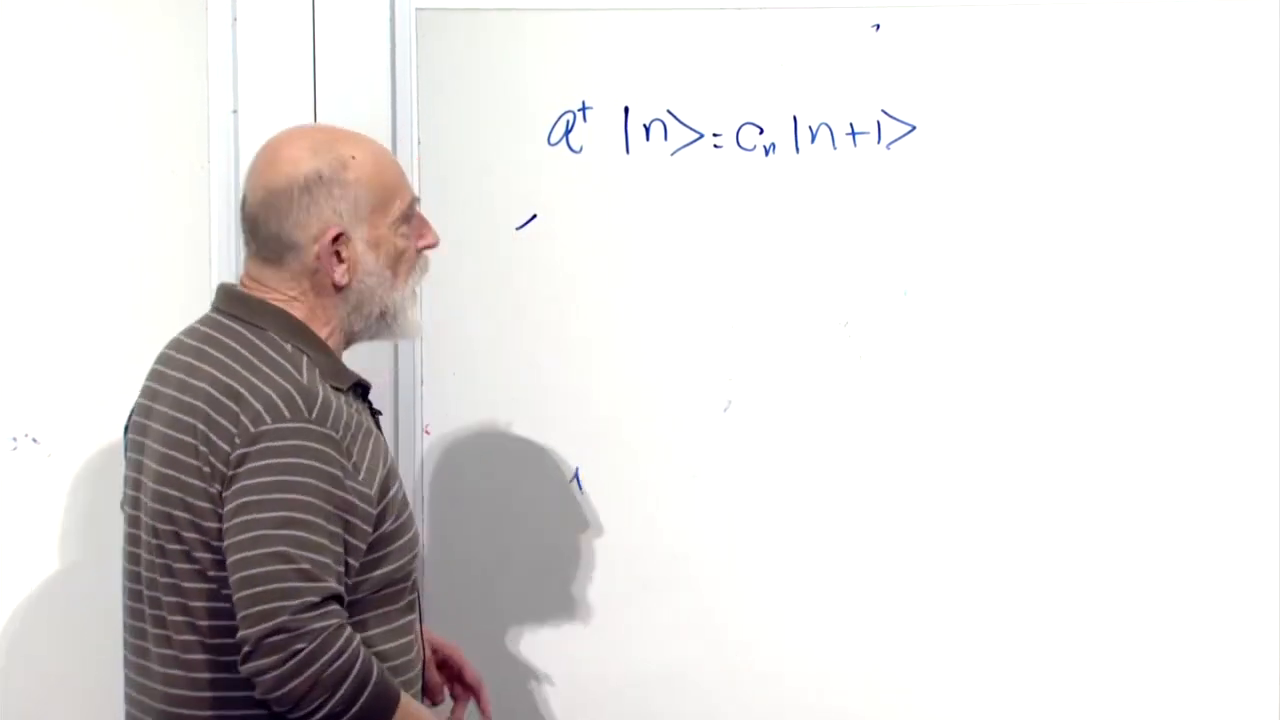
\includegraphics[width=0.9\linewidth]{lecture_06_frame_01.png}
\caption{يُدخَل معامل السلم قبل اشتقاق تطبيعه. وتُعاد كتابة المعادلة المكتوبة على اللوح في المعادلة~\eqref{eq:l06-unknown-coefficient}.}
\lectureframe{00:19:38}
\end{figure}

نختار اصطلاح الطور الذي يكون فيه \(c_n\) حقيقيًا. ويعطي أخذ المرافق الهيرميتي
\begin{equation}
\langle n|a=c_n\langle n+1|.
\end{equation}
وبضرب العلاقتين واستعمال حالات أساس مطبَّعة، نحصل على
\begin{align}
c_n^2
&=\langle n|aa^\dagger|n\rangle \\
&=\langle n|(a^\dagger a+1)|n\rangle \\
&=\langle n|(N+1)|n\rangle \\
&=n+1.
\end{align}
وبالتالي،
\begin{equation}
a^\dagger|n\rangle=\sqrt{n+1}\,|n+1\rangle.
\label{eq:l06-raising-rule}
\end{equation}

\begin{classroomqa}
\lecturetimestamp{00:22:35}
\audiencequestion{لماذا يجوز وضع \(\langle n+1|n+1\rangle=1\) قبل إيجاد \(c_n\)؟}
\lecturerresponse{تُختار المتجهات الذاتية منذ البداية على أنها أساس مطبَّع. ولا يحدد تطبيعها تطبيع \(a^\dagger|n\rangle\)؛ وهذه المعلومة المتبقية هي بالضبط المعامل \(c_n\).}
\end{classroomqa}

وتنتج قاعدة الخفض بالطريقة نفسها:
\begin{equation}
a|n\rangle=\sqrt n\,|n-1\rangle.
\label{eq:l06-lowering-rule}
\end{equation}
وعند \(n=0\)، ينعدم المعامل تلقائيًا، ولذلك تتضمن القاعدة \(a|0\rangle=0\). ومع وجود أنماط كثيرة، لا يغير المؤثر إلا عدد الإشغال في خانته الخاصة:
\begin{align}
a_i^\dagger|n_1,\ldots,n_i,\ldots\rangle
&=\sqrt{n_i+1}\,|n_1,\ldots,n_i+1,\ldots\rangle, \\
a_i|n_1,\ldots,n_i,\ldots\rangle
&=\sqrt{n_i}\,|n_1,\ldots,n_i-1,\ldots\rangle.
\label{eq:l06-multimode-ladders}
\end{align}
ولا يحدث شيء للخانات الأخرى.

\section{الدالة الموجية ليست حقلًا كموميًا}

قبل تعريف الحقل، علينا أن نميّزه عن الدالة الموجية المألوفة. وثلاثة أوجه تباين تنظّم هذا الانتقال.

أولًا، إن دالة موجية لجسيم واحد
\begin{equation}
\psi(x)=\langle x|\psi\rangle
\end{equation}
هي تمثيل لمتجه حالة. وهي ليست بنفسها كمية قابلة للرصد. فنحن نقيس الموضع، والزخم، والعزم الزاوي، وغير ذلك من المؤثرات؛ والدالة الموجية تزودنا بالسعات التي تُحسب منها احتمالات تلك النواتج.

ثانيًا، تعتمد الدالة الموجية لكثير من الجسيمات على مواضع جميع الجسيمات. وبالنسبة إلى جسيمين يُسمى متجها موضعيهما مؤقتًا \(x\) و\(y\)، يكون لدينا
\begin{equation}
\psi(x,y)=\langle x,y|\psi\rangle.
\end{equation}
وهنا يشير \(x\) و\(y\) إلى جسيمين مختلفين؛ وليسا المركبتين الديكارتيتين \(x\) و\(y\) لمتجه موضع واحد. ومع وجود \(N\) جسيمات، تُمثَّل الحالة بـ
\begin{equation}
\psi(x_1,x_2,\ldots,x_N).
\end{equation}

ثالثًا، تصف هذه الدالة الموجية عددًا ثابتًا من الجسيمات. فالدالة الموجية لخمسة عشر جسيمًا لها خمسة عشر وسيطًا موضعيًا، وتنتمي إلى فضاء هيلبرت لخمسة عشر جسيمًا. وهي لا تصف بذاتها عملية يتغير فيها العدد من خمسة عشر إلى أربعة عشر أو ستة عشر.

سيعكس الحقل الكمي هذه السمات. فهو مؤثر لا حالة، ويعتمد على نقطة مكانية واحدة \(x\)، ويؤثر في فضاء حالات يحتوي كل قطاع من قطاعات عدد الجسيمات. ويعني التعبير ``نقطة واحدة'' متجه موضع واحدًا متغيرًا بحرية. ولا يعني أن \(x\) قد أُسنِدت إليه قيمة عددية واحدة.

وهناك قيد واحد سيهم لاحقًا. فالحقل \(\Psi(x)\) الذي سيُدخَل أدناه ليس هيرميتيًا، ولذلك فهو ليس بنفسه كمية قابلة للرصد بالمعنى الصارم. أما تراكيبه الهيرميتية فهي كميات قابلة للرصد. ومن ثم فإن العبارة المؤقتة القائلة إن الحقل قابل للقياس تُصقل ولا تُطرح جانبًا: فالحقول دوال ذات قيم مؤثرية، وتراكيبها الهيرميتية تمثل كميات قابلة للقياس.

\begin{classroomqa}
\lecturetimestamp{00:36:52}
\audiencequestion{إذا كان الحقل دالة في موضع واحد، فهل يجوز لذلك الموضع أن يتغير؟ وماذا حدث لـ \(y\) في الدالة الموجية ذات الجسيمين؟}
\lecturerresponse{تتغير النقطة \(x\) على امتداد الفضاء كله. إن ``موضعًا واحدًا'' يعني أن للمؤثر وسيطًا مكانيًا واحدًا، لا أن هذا الوسيط ثابت. وفي \(\psi(x,y)\)، يسمي الرمزان \(x\) و\(y\) موضعي جسيمين؛ وبصورة مكافئة هما \(x_1\) و\(x_2\). وليسا مركبتين ديكارتيتين لوسيط الحقل.}
\end{classroomqa}

\begin{classroomqa}
\lecturetimestamp{00:38:15}
\audiencequestion{كيف يرتبط وصف الدالة الموجية ذات العدد الثابت من الجسيمات بوصف الحقل، وهل يصفان أنواعًا مختلفة من الجسيمات؟}
\lecturerresponse{هذا الارتباط هو البنية المركزية التي لم تأت بعد. والجسيمات من النوع نفسه. وفي هذه المحاضرة هي بوزونات؛ أما الفرميونات فتتطلب جبرًا مختلفًا.}
\end{classroomqa}

\section{جسيم واحد في صندوق}

لنعد مؤقتًا إلى ميكانيكا الكم العادية لجسيم واحد. ضع جسيمًا في صندوق أحادي البعد. ومع وجود جسيم واحد فقط، يصبح التمييز بين البوزون والفرميون غير ذي صلة: إذ لا يوجد جسيم مطابق ثانٍ يمكن به اختبار التبادل أو الاستبعاد.

لتكن
\begin{equation}
\psi_1(x),\ \psi_2(x),\ \psi_3(x),\ldots
\end{equation}
هي الدوال الذاتية للطاقة. فالنمط الأدنى هو أكثر موجة سلاسةً وتنعدم عند الجدران. وللنمط التالي عقدة داخلية واحدة، أما الأنماط الأعلى طاقة فتتذبذب بسرعة أكبر. وفي البئر المربعة اللانهائية المثالية ذات العرض \(L\)، فإن أساسًا مطبَّعًا مناسبًا هو
\begin{equation}
\psi_i(x)=\sqrt{\frac{2}{L}}\sin\!\left(\frac{i\pi x}{L}\right),
\qquad 0<x<L.
\label{eq:l06-box-basis}
\end{equation}
وصيغة الجيب الصريحة هذه تجسيد قياسي للرسم التخطيطي النوعي على اللوح؛ أما الحجة أدناه فلا تتطلب إلا مجموعة كاملة متعامدة ومتطبعة من حالات الجسيم الواحد.

\begin{figure}[htbp]
\centering
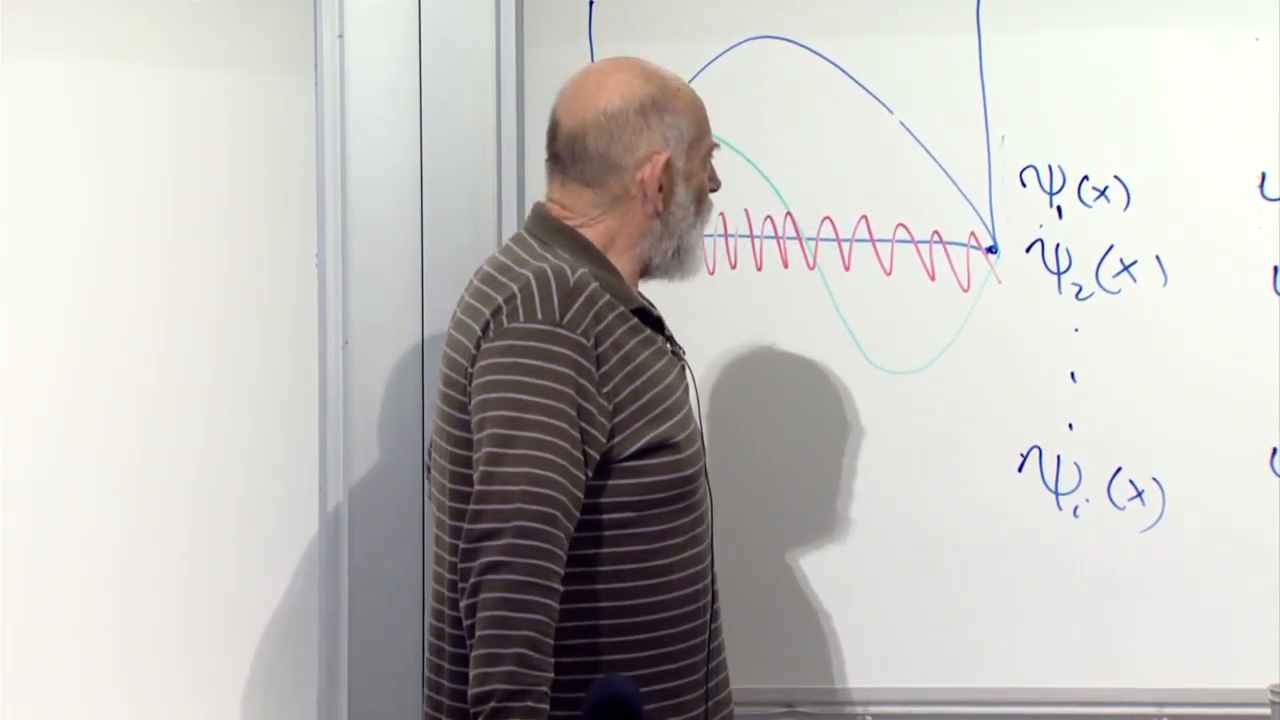
\includegraphics[width=0.9\linewidth]{lecture_06_frame_03.png}
\caption{أنماط الصندوق لجسيم واحد مرتبة بحسب تزايد الطاقة. لا يحتوي النمط الأول على أي عقدة داخلية، ويحتوي الثاني على عقدة واحدة، أما الأنماط الأعلى المحذوفة فتتذبذب بسرعة أكبر على نحو متزايد.}
\lectureframe{00:43:10}
\end{figure}

يمكن إعادة رسم البنية نفسها من دون الحجب الذي تسببه السبورة أثناء المحاضرة:
\begin{figure}[htbp]
\centering
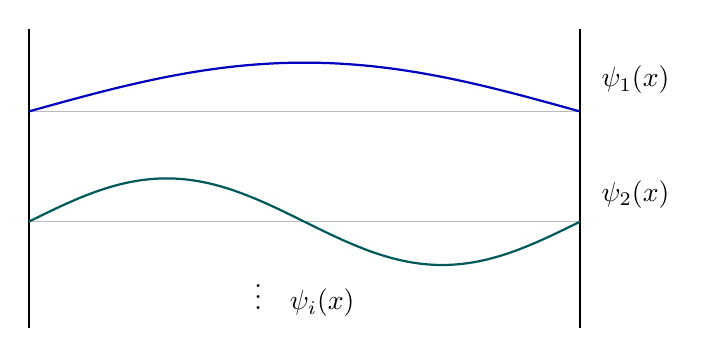
\begin{tikzpicture}[x=1cm,y=1cm]
  \draw[thick] (0,0) -- (0,3.8);
  \draw[thick] (7,0) -- (7,3.8);
  \draw[gray!55] (0,2.75) -- (7,2.75);
  \draw[gray!55] (0,1.35) -- (7,1.35);
  \draw[blue!75!black,thick,domain=0:7,samples=120]
    plot (\x,{2.75+0.62*sin(180*\x/7)});
  \draw[teal!70!black,thick,domain=0:7,samples=120]
    plot (\x,{1.35+0.55*sin(360*\x/7)});
  \node[right] at (7.15,3.15) {$\psi_1(x)$};
  \node[right] at (7.15,1.70) {$\psi_2(x)$};
  \node at (3.5,0.45) {$\vdots\quad \psi_i(x)$};
\end{tikzpicture}
\caption{إعادة بناء نظيفة للرسم التخطيطي الكيفي لأنماط الصندوق. تفصل الإزاحة العمودية بين الدوال الذاتية لتسهيل القراءة، وليست إحداثيًا فيزيائيًا إضافيًا.}
\end{figure}

يشير الدليل \(i\) إلى حالة أحادية الجسيم، لا إلى جسيم ولا إلى عدد العقد. وفي أساس الصندوق، يصادف أن يكون \(i\) أكبر بواحد من عدد العقد الداخلية. ولكل حالة طاقة \(\varepsilon_i\). واتباعًا لترميز المحاضرة، يمكننا أن نكتب هذه الطاقة على صورة \(\hbar\omega_i\)، أو ببساطة \(\omega_i\) بعد وضع \(\hbar=1\).

\begin{classroomqa}
\lecturetimestamp{00:39:01}
\audiencequestion{هل كان افتراض الاستقلال السابق دقيقًا تمامًا، وهل يمكن أن يوسم الدليل \(i\) الحالات الممكنة لإلكترون في ذرة؟}
\lecturerresponse{في بناء الأنماط المستقلة تكون علاقات الإبدال بين الأنماط المختلفة دقيقة تمامًا. ويمكن للدليل أن يوسم حالات ذرية أحادية الجسيم. أما إذا تفاعلت الجسيمات، فإن هاملتوني الأنماط المستقلة البسيط لا يعود هو الوصف الكامل.}
\end{classroomqa}

\begin{classroomqa}
\lecturetimestamp{00:40:34}
\audiencequestion{هل الجسيم في الصندوق بوزون؟}
\lecturerresponse{قد يكون كذلك، لكن مع جسيم واحد لا يهم الإحصاء. ولا يكتسب الاستبعاد والتبادل معنى إلا عندما يوجد أكثر من جسيم متماثل واحد.}
\end{classroomqa}

\section{من أنماط الصندوق إلى فضاء فوك}

لنسمح الآن بأي عدد من البوزونات المتماثلة في الصندوق. قد يشغل عدد ما \(n_1\) الحالة \(\psi_1\)، وقد يشغل عدد ما \(n_2\) الحالة \(\psi_2\)، وهكذا. ومن ثم تكون حالة أساس هي
\begin{equation}
|n_1,n_2,n_3,\ldots\rangle.
\end{equation}
وهذا هو بالضبط الترميز المستخدم من قبل لعدد كبير من المهتزات. والتطابق هنا بنيوي: اربط مهتزًا واحدًا بكل حالة أحادية الجسيم، واعتبر عدد إثارة المهتز هو عدد الجسيمات التي تشغل تلك الحالة.

البوزونات أساسية هنا لأن كل \(n_i\) يمكن أن يكون أي عدد صحيح غير سالب. أما في حالة الفرميونات، فكل حالة أحادية الجسيم يمكن أن تكون فارغة أو مشغولة بجسيم واحد فقط، ولا يمكن أن تكون مشغولة بجسيمين، لذلك لا يمكن استعمال جبر المهتز المعتاد من غير تعديل.

يمكن الآن تعريف المؤثرات من خلال فعلها على أساس أعداد الإشغال. فالمؤثر \(a_i^\dagger\) يخلق جسيمًا واحدًا في الحالة أحادية الجسيم \(i\)؛ و\(a_i\) يزيل جسيمًا واحدًا:
\begin{align}
a_i^\dagger|n_1,\ldots,n_i,\ldots\rangle
&=\sqrt{n_i+1}\,|n_1,\ldots,n_i+1,\ldots\rangle, \\
a_i|n_1,\ldots,n_i,\ldots\rangle
&=\sqrt{n_i}\,|n_1,\ldots,n_i-1,\ldots\rangle.
\end{align}
وليست هذه مجرد مماثلة لاحقة. بل هذا هو تعريف مؤثري الخلق والفناء البوزونيين على هذا الأساس. وبما أن هذا الأساس يمتد على الفضاء، فإن التعريف يحدد فعلهما على كل حالة بالخطية.

\begin{classroomqa}
\lecturetimestamp{00:47:11}
\audiencequestion{هل \(n_1,n_2,n_3\) هي الحالات الكمومية؟}
\lecturerresponse{تحدد الوسوم \(1,2,3,\ldots\) الحالات أحادية الجسيم. أما الرموز \(n_1,n_2,n_3,\ldots\) فهي أعداد الجسيمات التي تشغل تلك الحالات. والحفاظ على التمييز بين وسم الحالة وعدد إشغالها هو العبء الترميزي الرئيسي.}
\end{classroomqa}

\subsection{ما الذي يفعله الجذر التربيعي}

العامل \(\sqrt{n_i+1}\) لا يمثل جسيمًا إضافيًا ولا عملية فيزيائية منفصلة. بل يمنح المؤثر التطبيع الصحيح والبنية الجبرية الصحيحة. وفي نمط واحد،
\begin{align}
a a^\dagger|n\rangle
&=a\bigl(\sqrt{n+1}\,|n+1\rangle\bigr) \\
&=(n+1)|n\rangle,
\end{align}
بينما
\begin{equation}
a^\dagger a|n\rangle=n|n\rangle.
\end{equation}
ومن ثم يكون الفرق بينهما هو \(|n\rangle\)، كما تقتضيه \([a,a^\dagger]=1\). وعلى نحو تقريبي جدًا، يكون كل من مؤثري السلم من رتبة \(\sqrt n\)، لأن حاصل ضربهما يعطي مؤثر العدد من رتبة \(n\).

\begin{classroomqa}
\lecturetimestamp{00:47:52}
\audiencequestion{ما المعنى الفيزيائي الملموس لعامل الجذر التربيعي؟}
\lecturerresponse{إنه في المقام الأول تطبيع رياضي. فهو يضمن أن حالات الإشغال مطبعة، وأن \(a^\dagger a\) له القيمة الذاتية \(n\)، وأن مؤثري السلم يحققان علاقة إبدال المهتز. أحيانًا تكون الرياضيات هي المعنى الذي نحتاج إليه.}
\end{classroomqa}

\begin{classroomqa}
\lecturetimestamp{00:52:25}
\audiencequestion{هل جرى تعريف مؤثري الخلق والفناء فقط من خلال خواصهما وفعلهما على الأساس؟}
\lecturerresponse{نعم. لا يلزم أن تنشأ التعريفات من تصور أكثر بدائية. وتختبر قيمتها بنتائجها. إن تعريف الفعل على أساس كامل يحدد المؤثرات على فضاء فوك كله، وهذه التعريفات تعيد إنتاج علاقات الإبدال المطلوبة.}
\end{classroomqa}

\begin{classroomqa}
\lecturetimestamp{00:53:22}
\audiencequestion{لماذا يجعل \(a_i\) جسيمًا يختفي بدلًا من أن ينقله فحسب إلى حالة مختلفة؟}
\lecturerresponse{لأن \(a_i\) معرَّف على أنه ينقص إشغال الحالة \(i\). والسؤال المفيد ليس لماذا يكون التعريف صحيحًا، بل لماذا يكون مفيدًا. وهو مفيد لأن الانبعاث والامتصاص يتطلبان مؤثرات تغيّر عدد الجسيمات: فالفوتون يُخلَق عند انبعاث الإشعاع ويُفنى عند امتصاصه.}
\end{classroomqa}

الفضاء الممتد بواسطة جميع حالات أعداد الإشغال هو \emph{فضاء فوك}. وهو يحتوي على الخلاء، وكل حالة أحادية الجسيم، وكل حالة ثنائية الجسيم، وهكذا من غير حد أعلى ثابت:
\begin{equation}
\mathcal F=\mathcal H_0\oplus\mathcal H_1\oplus\mathcal H_2\oplus\cdots.
\label{eq:l06-fock-space}
\end{equation}
ويُظهر ترميز المجموع المباشر صراحةً ما لم تُظهره دالة الموجة المعتادة ذات \(N\) جسيمًا: فجميع قطاعات عدد الجسيمات تنتمي إلى فضاء حالة واحد.

\begin{classroomqa}
\lecturetimestamp{00:54:56}
\audiencequestion{هل يؤدي تعريف المؤثرات على المتجهات الذاتية لعدد الإشغال إلى تحديدها على متجهات اعتباطية، وهل تتبع بعد ذلك علاقات إبدال المهتز؟}
\lecturerresponse{بالضبط. فمتجهات الإشغال تشكل أساسًا، لذا تمد الخطية التعريف إلى فضاء فوك كله. والتحقق من علاقات الإبدال البوزونية يتم بفعل المؤثرات على ذلك الأساس. وتمثل كل حالة أحادية الجسيم بمهتز واحد، ويكون إشغال ذلك المهتز هو عدد الجسيمات في تلك الحالة.}
\end{classroomqa}

\subsection{الخلاء والهاملتوني الحر}

خلاء فوك هو الحالة التي لا يوجد فيها أي جسيم في أي حالة أحادية الجسيم:
\begin{equation}
|0\rangle=|0,0,0,\ldots\rangle,
\qquad a_i|0\rangle=0.
\end{equation}
وقد تكون كلمة \emph{الحالة القاعية} مضللة هنا. فأدنى حالة \emph{أحادية الجسيم} هي النمط \(i=1\)؛ ولا يوجد في خلاء فوك أي جسيم حتى في ذلك النمط. وإذا شغل جسيم النمط الأدنى، أمكن لـ \(a_1\) أن يزيله ويعيد النظام إلى الخلاء.

\begin{classroomqa}
\lecturetimestamp{00:56:19}
\audiencequestion{ما الخلاء بلغة عدد الإشغال؟ وهل تكون أدنى حالة أحادية الجسيم مشغولة؟}
\lecturerresponse{في الخلاء يكون كل عدد إشغال مساويًا للصفر، ويفنيه كل \(a_i\). وأدنى نمط أحادي الجسيم غير مشغول في الخلاء. ولو كان مشغولًا، لأمكن لمؤثر إفنائه أن يزيل ذلك الجسيم.}
\end{classroomqa}

بالنسبة إلى الجسيمات غير المتفاعلة، تكون الطاقة الكلية هي مجموع المساهمات. فإذا كانت طاقة جسيم واحد في الحالة \(i\) هي \(\hbar\omega_i\)، فإن
\begin{align}
H
&=\sum_i \hbar\omega_i N_i \\
&=\sum_i \hbar\omega_i a_i^\dagger a_i.
\label{eq:l06-free-fock-hamiltonian}
\end{align}
وهناك قراءتان متكافئتان لذلك. فهو مجموع طاقات المهتزات، مهتز واحد لكل حالة أحادية الجسيم. وهو أيضًا مجموع الطاقات أحادية الجسيم، مضروبةً كل منها في عدد الجسيمات التي تحمل تلك الطاقة.

في ترميز نظرية الحقل، يُسمَّى \(a_i^\dagger\) عادةً مؤثر الخلق، ويُسمَّى \(a_i\) مؤثر الفناء. أما الترميز الأقدم \(a_+\) و\(a_-\) فيعني الشيء نفسه.

\section{توضيحات قبل أن يظهر الحقل}

تُميِّز عدة أسئلة بعد الاستراحة بين طريقة تتبّع المهتزات الجديدة هذه وبين جسيم عادي يتحرك في كمون مهتز.

\begin{classroomqa}
\lecturetimestamp{01:06:09}
\audiencequestion{إن مستويات طاقة جسيم في صندوق ليست متساوية التباعد، فأين المهتز التوافقي؟}
\lecturerresponse{لا يلزم أن تكون الطاقات أحادية الجسيم \(\omega_i\) متساوية التباعد. لكن، لكل نمط ثابت \(i\)، تكون طاقات صفر جسيم، وجسيم واحد، وجسيمين، وثلاثة جسيمات غير متفاعلة في ذلك النمط هي \(0,\omega_i,2\omega_i,3\omega_i\). وذلك سلّم الإشغال هو المهتز. وهو يختلف عن وضع جسيم واحد في كمون مهتز توافقي.}
\end{classroomqa}

\begin{classroomqa}
\lecturetimestamp{01:08:38}
\audiencequestion{هل يرتبط هذا البناء بتحليل فورييه؟}
\lecturerresponse{على نحو عميق. فإذا كان الأساس الأحادي الجسيم يتكوّن من أنماط الزخم، كانت دوال الأنماط جيوبًا، أو جيوب تمام، أو أسّيات مركبة، وكانت \(a_i\) نظائر كمومية لمعاملات فورييه. وليس من الضروري أن يكون أساس عام مثلثيًا، لكن منطق التوسيع هو نفسه.}
\end{classroomqa}

\begin{classroomqa}
\lecturetimestamp{01:09:07}
\audiencequestion{هل تُسنَد الطاقة نفسها إلى جميع الجسيمات، وهل أُدرجت التفاعلات؟}
\lecturerresponse{الجسيمات التي تشغل الحالة الأحادية نفسها تكون لها الطاقة نفسها، بينما الجسيمات في حالات مختلفة لا تكون كذلك في العموم. وفي الوقت الحالي الجسيمات حرة: فهي لا تتفاعل. وستضيف التفاعلات حدود طاقة وضع، ولذلك لن يعود الهاملتوني مجرد المجموع الجمعي في المعادلة~\eqref{eq:l06-free-fock-hamiltonian}.}
\end{classroomqa}

\begin{classroomqa}
\lecturetimestamp{01:10:26}
\audiencequestion{ماذا حلّ بنصف كمّ طاقة نقطة الصفر في كل مهتز؟}
\lecturerresponse{إنه ثابت إضافي في الهاملتوني. والثابت يتبادل مع كل مؤثر، لذا فهو لا يغيّر معادلات الحركة لهايزنبرغ، كما أن القياسات المعتادة غير الثقالية تعتمد على فروق الطاقة. وقد تكون له أهمية لأغراض خاصة، لكنه لا يؤثر في البناء الذي نطوره هنا.}
\end{classroomqa}

إن النظرية الحرة هي بالفعل أداة لتتبّع الحسابات ذات قدرة غير مألوفة. فهي تتتبّع لا جسيمات كثيرة فحسب، بل أيضًا جسيمات تغيّر حالتها، أو تظهر، أو تختفي، أو توجد في تراكبات لأعداد كلية مختلفة. والمؤثرات أكثر من مجرد رموز في هذا التتبّع، لأن تراكيب هيرميتية مناسبة يمكن قياسها، لكن هذه الفكرة تظل حدسًا أوليًا مفيدًا.

\begin{classroomqa}
\lecturetimestamp{01:14:03}
\audiencequestion{من أين جاءت نظرية الحقل ونظرية الحقل الكمومي تاريخيًا؟}
\lecturerresponse{يبدأ مسار تاريخي موجز بصورة فاراداي الفيزيائية للحقول الكهربائية والمغناطيسية، ومعادلات ماكسويل للحقول الكلاسيكية. وقدّم بلانك كمّات الطاقة أثناء دراسته للإشعاع الحراري؛ وربط آينشتاين هذا التكميم بالحقل الكهرومغناطيسي نفسه وبكمّات الضوء. ثم ساعد هايزنبرغ وباولي، وبخاصة ديراك، في تجميع الإطار المؤثري الحديث قرب نهاية عقد 1920. وكانت الكارثة فوق البنفسجية والوصف الكمومي للإشعاع من بين المشكلات المبكرة الحاسمة. وهذه صورة تاريخية تخطيطية لا إسناد كامل فيها للأسبقية.}
\end{classroomqa}

ويفسر الخيط التاريخي أيضًا سبب تكرر ظهور المهتزات. فالإشعاع الكلاسيكي في تجويف يتحلل إلى أنماط عادية. وتكميم تلك الأنماط يحوّل أعداد إثارتها إلى أعداد فوتونات. والكمّات الرياضية التي تشغل الأنماط تصبح جسيمات فيزيائية.

\section{مؤثر الحقل البوزوني}

لتكن \(\{\psi_i(x)\}\) أساسًا كاملًا متعامدًا ومطبَّعًا لدوال موجة الجسيم الواحد. عرّف
\begin{equation}
\boxed{\Psi(x)=\sum_i a_i\,\psi_i(x)}
\label{eq:l06-field-annihilation}
\end{equation}
ومرافقه الهيرميتي
\begin{equation}
\boxed{\Psi^\dagger(x)=\sum_i a_i^\dagger\,\psi_i^*(x)}.
\label{eq:l06-field-creation}
\end{equation}

\begin{figure}[htbp]
\centering
\includegraphics[width=0.9\linewidth]{lecture_06_frame_04.png}
\caption{التوسعات النمطية المكتملة لحقل الإبادة ولمرافقه الهيرميتي. وتحافظ المعادلتان~\eqref{eq:l06-field-annihilation} و\eqref{eq:l06-field-creation} في التنضيد على البنية نفسها من حيث المؤثر والاقتران العقدي.}
\lectureframe{01:25:15}
\end{figure}

عند أي موضع ثابت \(x\)، تكون كل \(\psi_i(x)\) عددًا مركبًا عاديًا. ويكمن كل المحتوى المؤثري في \(a_i\) و\(a_i^\dagger\). ومع تغيّر \(x\)، نحصل على مؤثر مختلف عند كل نقطة في الفضاء. وهذا هو المعنى الدقيق الذي تكون به \(\Psi\) دالةً قيمُها مؤثرات.

إذا كانت دوال الأساس موجات مستوية، فإن المعادلتين~\eqref{eq:l06-field-annihilation} و\eqref{eq:l06-field-creation} تمثلان توسعهَي فورييه كمّيين: فقد أصبحت معاملات فورييه الكلاسيكية مؤثرات. وفي صندوق، قد يكون الأساس بدلًا من ذلك دوال الجيب في المعادلة~\eqref{eq:l06-box-basis}. ويصلح أي أساس كامل متعامد ومطبَّع للجسيم الواحد.

ليس أيٌّ من \(\Psi\) و\(\Psi^\dagger\) هيرميتيًا. ويمكن بناء حقول قابلة للرصد من تراكيب هيرميتية مثل
\begin{equation}
\Psi(x)+\Psi^\dagger(x),
\qquad
i\bigl(\Psi^\dagger(x)-\Psi(x)\bigr),
\end{equation}
وستُبنى الكثافات القابلة للرصد لاحقًا من جداءات مثل \(\Psi^\dagger(x)\Psi(x)\). والمهمة الحالية هي أن نفهم أولًا ما الذي يفعله الحقلان الأساسيان.

\begin{classroomqa}
\lecturetimestamp{01:23:14}
\audiencequestion{كيف يمكن أن يكون الطرف الأيسر مؤثِّرًا بينما دوال الأنماط في الطرف الأيمن دوال موجية عادية؟}
\lecturerresponse{تصبح الدوال \(\psi_i(x)\) أعدادًا بمجرد اختيار \(x\). أما العوامل \(a_i\) فهي مؤثِّرات. والعدد المضروب في مؤثِّر هو مؤثِّر، ولذلك يكون المجموع مؤثِّرًا. ومع تغيير \(x\) نحصل على العائلة الكاملة من المؤثِّرات.}
\end{classroomqa}

\section{ما يفعله الحقل}

حقل الإفناء يُفني حالة الفراغ فورًا:
\begin{equation}
\Psi(x)|0\rangle
=\sum_i\psi_i(x)a_i|0\rangle
=0.
\label{eq:l06-field-kills-vacuum}
\end{equation}
أما حقل الخلق فيفعل شيئًا أكثر إفادة بكثير.

لتدل \(|i\rangle\) على حالة الجسيم الواحد ذات الدالة الموجية
\begin{equation}
\langle x|i\rangle=\psi_i(x).
\end{equation}
فإن اكتمال أساس الجسيم الواحد يعطي
\begin{equation}
\sum_i|i\rangle\langle i|=1.
\label{eq:l06-completeness}
\end{equation}
طبِّق هذه المتطابقة على حالة ذاتية للموضع:
\begin{align}
|x\rangle
&=\sum_i|i\rangle\langle i|x\rangle \\
&=\sum_i\psi_i^*(x)|i\rangle.
\label{eq:l06-position-expansion}
\end{align}
وفي لغة فوك، تكون حالة النمط أحادي الجسيم
\begin{equation}
|i\rangle=a_i^\dagger|0\rangle.
\end{equation}
وبالتعويض بهذا في المعادلة~\eqref{eq:l06-position-expansion}،
\begin{align}
|x\rangle
&=\sum_i\psi_i^*(x)a_i^\dagger|0\rangle \\
&=\Psi^\dagger(x)|0\rangle.
\label{eq:l06-local-creation}
\end{align}
ومن ثم فإن \(\Psi^\dagger(x)\) يخلق جسيمًا متموضعًا عند \(x\)، بينما يزيل \(\Psi(x)\) جسيمًا من هناك. وحالة الموضع الذاتية متمركزة بدالة دلتا، وهي حالة معمَّمة غير قابلة للتطبيع؛ أما الجسيم الفيزيائي المتموضع فيُحصَل عليه بتلطيخ الحقل بحزمة موجية قابلة للتطبيع.\editorialnote{تتحدث المحاضرة بلغة حالات الموضع الذاتية المثالية. ويسجِّل قيد الحزمة الموجية هذا المعنى الرياضي المعياري من غير أن يغيِّر الحجة.}

\begin{classroomqa}
\lecturetimestamp{01:36:26}
\audiencequestion{أين توجد المعلومة التي تحدد أيَّ نوع من الجسيمات يُخلَق؟ وهل الحالة عند \(x\) متمركزة بدالة دلتا؟}
\lecturerresponse{يُخصَّص حقل مستقل لكل نوع من الجسيمات، لذا تُحمَل هوية الجسيم بواسطة الحقل المستخدم. ويحدد الوسيط \(x\) الموضع الذي يُخلَق عنده. وفي أساس الموضع المثالي تكون الحالة المخلوقة متمركزة بدالة دلتا.}
\end{classroomqa}

من أمثلة الأنواع البوزونية الفوتونات والغرافيتونات وبوزونات هيغز والغلوونات، مع أن الحقول الواقعية تحمل أيضًا مؤشرات داخلية. وحتى الفوتونات تتطلب وسومًا للاستقطاب. ويحجب ترميز الحقل السلمي المبسَّط تلك الوسوم الإضافية لكي يظل مبدأ الخلق ظاهرًا.

\subsection{الفراغ ليس المتجه الصفري}

المعادلة
\begin{equation}
\Psi(x)|0\rangle=0
\end{equation}
تتضمن شيئين مختلفين جدًا يُرمَز إليهما بالصفر. فالكيت \(|0\rangle\) هو الفراغ: حالة فيزيائية مطبَّعة تحقق
\begin{equation}
\langle0|0\rangle=1.
\end{equation}
أما الناتج في الطرف الأيمن فهو المتجه الصفري. معياره صفر؛ فلا يمكن تطبيعه ولا يمثِّل حالة فيزيائية.

يتضح الفرق بجلاء عند الجمع. فإضافة المتجه الصفري إلى حالة جسيم واحد لا تغيِّر شيئًا. أما إضافة الفراغ إلى حالة جسيم واحد فتعطي تراكبًا حقيقيًا لقطاعات مختلفة من عدد الجسيمات. ومع معاملات مطبَّعة،
\begin{equation}
|\chi\rangle=\frac{1}{\sqrt2}\bigl(|0\rangle+|1\rangle\bigr)
\end{equation}
له احتمالان متساويان لعدم وجود أي جسيم ووجود جسيم واحد. وليس هو نفسه \(|1\rangle\).

\begin{classroomqa}
\lecturetimestamp{01:37:23}
\audiencequestion{إذا لم يوجد أي جسيم عند \(x\)، فهل يكون \(\Psi(x)\) عندئذٍ لا يفعل شيئًا فحسب؟ وماذا يعني أن تكون النتيجة صفرًا؟}
\lecturerresponse{إنه لا يعيد الحالة الأصلية. بل يعيد المتجه الصفري. والفراغ حالة مطبَّعة تصف الفضاء الخالي؛ أما المتجه الصفري فطوله صفر ولا يصف أي حالة فيزيائية. وأي مؤثِّر يؤثر في المتجه الصفري يعيد المتجه الصفري.}
\end{classroomqa}

\begin{classroomqa}
\lecturetimestamp{01:39:00}
\audiencequestion{ماذا يحدث إذا أُضيفت حالة الفراغ بدلًا من متجه الصفر إلى حالة أحادية الجسيم؟}
\lecturerresponse{نحصل على تراكب له سعات لأعداد جسيمات مختلفة. وعلى النقيض من ذلك، فإن إضافة متجه الصفر تترك حالة الجسيم الواحد من دون تغيير. والرمز في \(|0\rangle\) يدل على إشغال صفري؛ ولا يعني متجه الصفر.}
\end{classroomqa}

\begin{classroomqa}
\lecturetimestamp{01:41:56}
\audiencequestion{هل يهم ترتيب دالة النمط ومؤثر إنشائها أو إفنائها في توسعة الحقل؟ وهل دوال الأنماط مركبة؟}
\lecturerresponse{دالة النمط عدد عادي، ولذلك فهي تتبادل مع كل مؤثر، لذا لا يهم الترتيب. وبوجه عام قد تكون دوال الأنماط مركبة؛ أمّا ما إذا كان أساس مختار حقيقيًا أم مركبًا فيعتمد على مسألة Schr\"odinger للجسيم الواحد.}
\end{classroomqa}

\subsection{جسيمان ونشوء التناظر البوزوني}

لإنشاء جسيم عند \(x\) وآخر عند \(y\)، نؤثر مرتين:
\begin{equation}
|x,y\rangle
=\Psi^\dagger(y)\Psi^\dagger(x)|0\rangle.
\label{eq:l06-two-particle-state}
\end{equation}
قد تتطابق النقطتان أو تختلفا. وبما أن مؤثرات الإنشاء الأساسية تتبادل،
\begin{align}
[\Psi^\dagger(x),\Psi^\dagger(y)]
&=\sum_{i,j}\psi_i^*(x)\psi_j^*(y)
[a_i^\dagger,a_j^\dagger] \\
&=0.
\end{align}
ويترتب على ذلك أن
\begin{equation}
\Psi^\dagger(y)\Psi^\dagger(x)|0\rangle
=\Psi^\dagger(x)\Psi^\dagger(y)|0\rangle.
\label{eq:l06-boson-exchange}
\end{equation}
إن تبديل ترتيب الجسيمين لا يغيّر شيئًا. وهذا هو بالضبط تناظر التبادل البوزوني. ولذلك كان يمكننا أن ننطلق من جبر المهتز وأن \emph{نستنتج} أن الجسيمات المشيدة من مؤثرات إنشاء متبادلة هي بوزونات. أمّا الفرميونات فستلزم بدلًا من ذلك مؤثرات متضادة التبادل.

\begin{classroomqa}
\lecturetimestamp{01:42:37}
\audiencequestion{كيف يُضاف جسيم ثانٍ إلى حالة الجسيم الواحد؟}
\lecturerresponse{طبّق حقل إنشاء آخر. ولإضافته عند \(y\)، نؤثر بـ \(\Psi^\dagger(y)\) إلى يسار \(\Psi^\dagger(x)\). والنتيجة هي حالة الجسيمين في المعادلة~\eqref{eq:l06-two-particle-state}.}
\end{classroomqa}

\begin{classroomqa}
\lecturetimestamp{01:46:04}
\audiencequestion{هل تبادلية حقلي الإنشاء مكافئة تمامًا لجعل حالة الجسيمين متناظرة؟}
\lecturerresponse{نعم. فهي تجعل الحالة التي فيها جسيم عند \(x\) وجسيم عند \(y\) مطابقة للحالة الناتجة بعد تبديل التسميتين. وهذه هي خاصية التبادل التعريفية للبوزونات المتطابقة.}
\end{classroomqa}

\begin{classroomqa}
\lecturetimestamp{01:46:32}
\audiencequestion{هل يعني هذا أن الجسيمات عند \(x\) و\(y\) يجب أن تكون من النوع نفسه من البوزونات؟}
\lecturerresponse{نعم. الوسيطان \(x\) و\(y\) هما موضعان، بينما يصف حقل واحد نوعًا واحدًا. وتتطلب الأنواع المختلفة، وكذلك الوسوم الإضافية مثل استقطابي الفوتون، مركبات حقلية متميزة.}
\end{classroomqa}

\section{لماذا يهمّ كون عدد الجسيمات متغيّرًا}

إذا كانت مسألة ما تحتوي على 37 جسيمًا بالضبط على الدوام، لكانت لغة الحقول مجرد تدوينٍ اختياري للتتبّع. وتظهر قوتها الحقيقية حين يمكن انبعاث الجسيمات وامتصاصها، وخصوصًا عندما يكون عدد الجسيمات نفسه متغيرًا كمّيًا. ويتيح فضاء فوك حالات من الشكل
\begin{equation}
|\Phi\rangle
=c_0|0\rangle+c_1|1\rangle+c_2|2\rangle+\cdots,
\qquad
\sum_{n=0}^{\infty}|c_n|^2=1.
\end{equation}
ويُعد حقل الليزر مثالًا مهمًا: فهو ليس عمومًا حالةً ذات عدد فوتونات محدد بدقة، بل تراكبًا من قطاعات عددية كثيرة.

أصبح الجسر بين الجسيمات والحقول الآن جليًّا. فمؤثرات الأنماط تحصي الجسيمات في الحالات الذاتية للطاقة وتغيّر عددها؛ ويجمع الحقل بين تلك المؤثرات ومجموعة كاملة من الدوال الموجية بحيث يمكن إنشاء الجسيمات أو إزالتها عند مواضع معيّنة. وقد أصبح جبر المهتزات التوافقية اللغة الأساسية لحقل كمّي بوزوني.
